\subsection*{Redigering af adgangskode} \label{sec:redigrering}
Ud fra app'ens hovedmenu har brugeren mulighed for at tilgå og få vist brugeroplysninger samt redigere sin adgangskode. Af \autoref{fig:Redigerbrugeroplysninger} illustreres aktivitetsdiagrammet for redigering af adgangskode.  

\begin{figure}[H]
\centering
\textbf{Aktivitetsdiagram: Redigering af adgangskode}\par\medskip
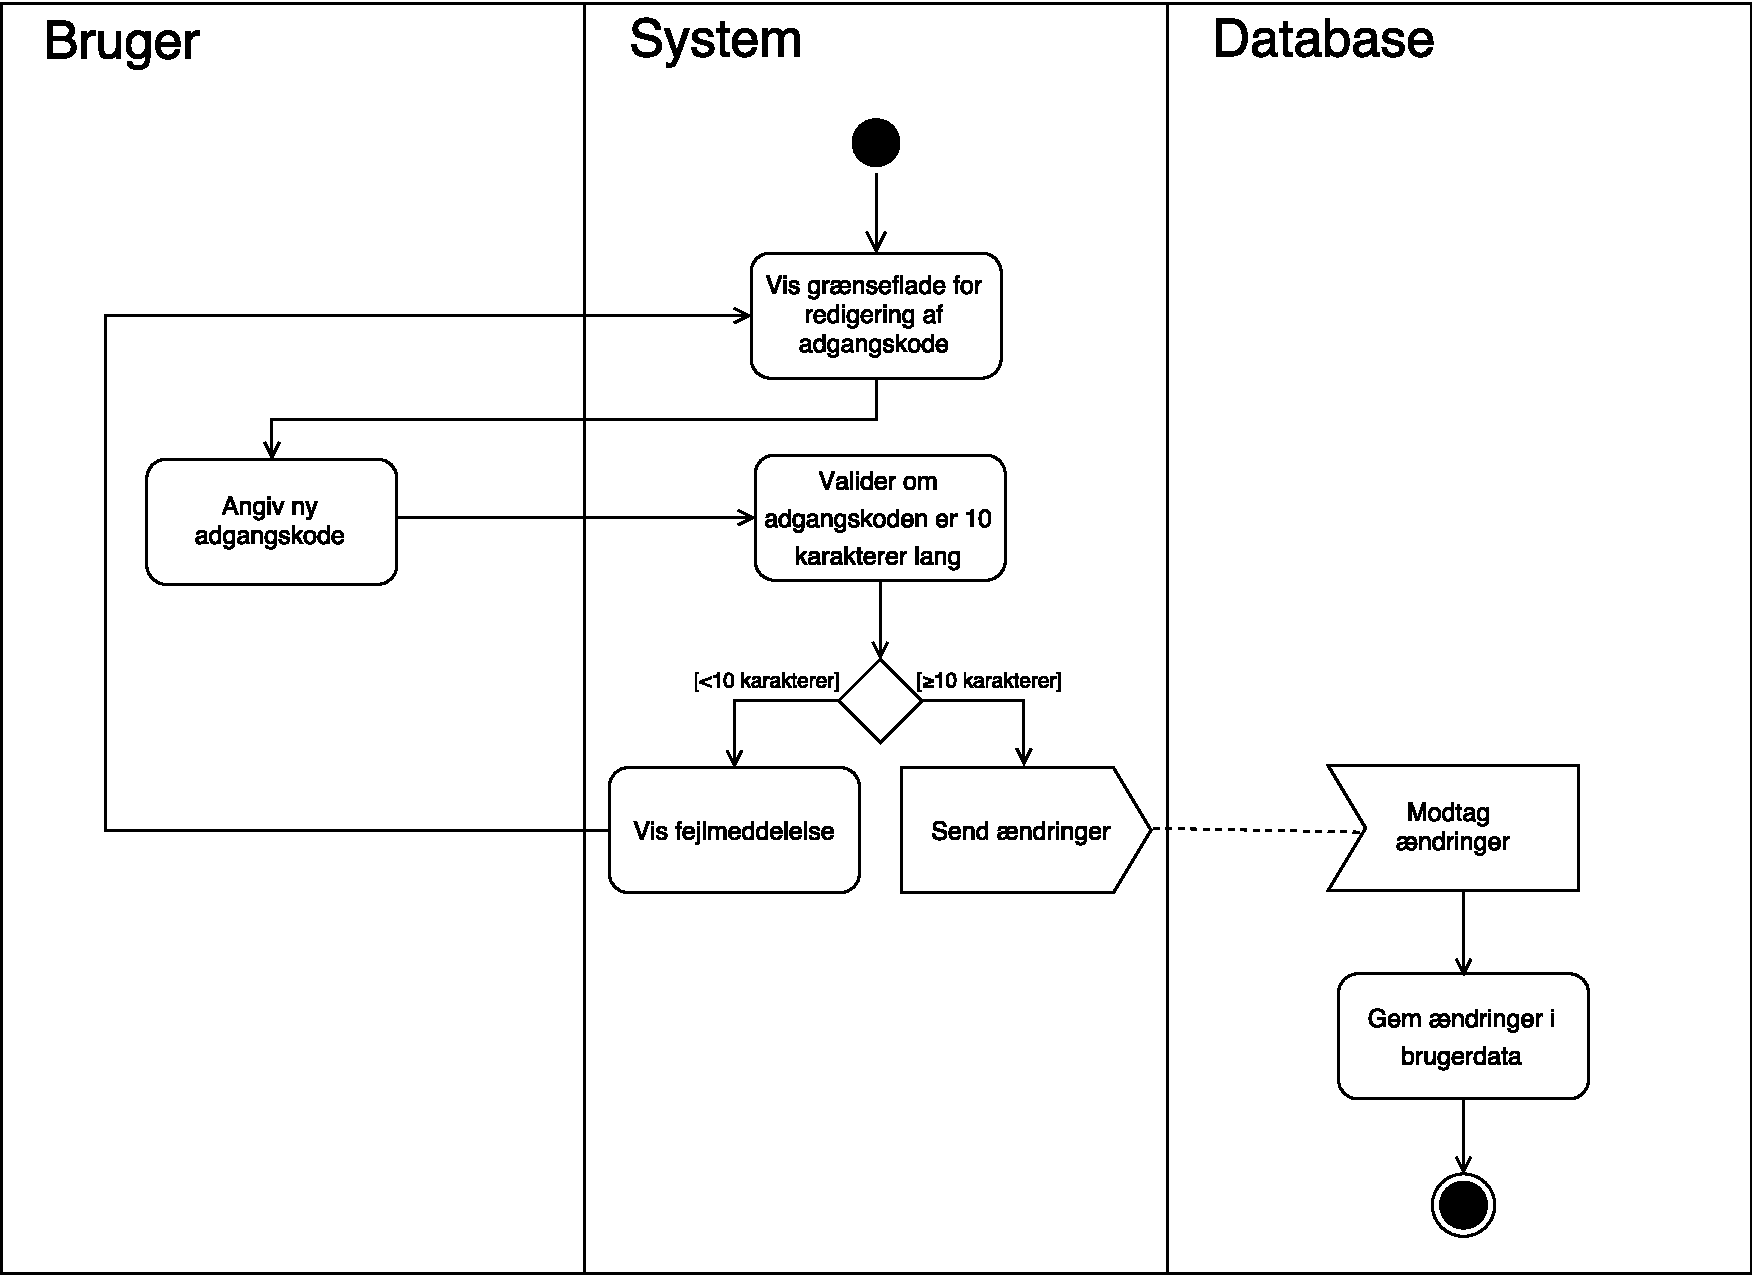
\includegraphics[width=1\textwidth]{figures/aktivitetsdiagram/Redigerbrugeroplysninger}
\caption{Aktivitetsdiagram for redigering af adgangskode.}
\label{fig:Redigerbrugeroplysninger}
\end{figure}

\noindent
Det skal være muligt for brugeren at ændre adgangskode, da brugeren ved oprettelse får tildelt en randomiseret adgangskode. Dertil kan adgangskoden blive personlig for brugeren, hvilket  vil gøre det nemmere for brugeren at huske. 
Brugeren kan ændre adgangskoden ved at vælge rediger adgangskode fra hovedmenuen, hvorefter grænsefladen for redigering af adgangskode vises.
For at den nye adgangskode kan benyttes, skal den minimum være 10 karakterer lang. Grunden til dette er, at der ved log ind sendes en fejlmeddelelse, hvis indtastede informationer ikke findes i databasen, dertil skal adgangskoden ikke kunne forveksles med fejlmeddelelsen. Desuden anbefaler Rådet for Digital Sikkerhed, at adgangskoder bør være minimum 10 karakterer lang, dog er dette ikke et krav \citep{sikkerhed2015}.
Hvis kravet om minimum 10 karakterer ikke opfyldes, sendes en fejlmeddelelse tilbage til brugeren, hvortil en ny adgangskode kan indtastes. 
Ændres adgangskoden sendes ændringen til databasen, hvorefter den gemmes i databasen.